%%%%%%%%%%%%%%%%%%%% MetalFish Paper %%%%%%%%%%%%%%%%%%%%%%%%%%%%%%%%%%%
%
% Hybrid Chess Search: Parallel Alpha-Beta and MCTS on Unified Memory
% IntelliSys 2026 -- Springer LNCS
%
%%%%%%%%%%%%%%%% Springer %%%%%%%%%%%%%%%%%%%%%%%%%%%%%%%%%%

\documentclass{svproc}

\usepackage{url}
\def\UrlFont{\rmfamily}
\usepackage{graphicx}
\usepackage{float}
\usepackage{placeins}
\usepackage{amsmath}
\usepackage{algorithm}
\usepackage{algpseudocode}
\usepackage{booktabs}
\usepackage{listings}
\usepackage{xcolor}
\usepackage{tikz}
\usepackage{pgfplots}
\usepackage{multirow}
\pgfplotsset{compat=1.18}
\usetikzlibrary{positioning, arrows.meta, shapes.geometric, fit, calc}
\newcommand{\stdmutex}{\texttt{std::\allowbreak mutex}}
\newcommand{\osunfairlock}{\texttt{os\_\allowbreak unfair\_\allowbreak lock}}

\begin{document}
\mainmatter

\title{Hybrid Chess Search: Combining Alpha-Beta and Monte Carlo Tree Search on Unified Memory Architectures}

\titlerunning{Hybrid Chess Search on Unified Memory}

% Author information
\author{Nripesh Niketan\thanks{ORCID: 0009-0008-2066-1937}}

\authorrunning{N. Niketan}

\institute{Independent Researcher\\
\email{nripesh14@gmail.com}}

\maketitle

% ===========================================================================
% ABSTRACT
% ===========================================================================

\begin{abstract}
We present a GPU-accelerated chess engine for Apple Silicon that integrates three search paradigms within a unified memory architecture: (1)~an alpha-beta engine with NNUE evaluation achieving 7.6M nodes per second on 8~threads, (2)~a Monte Carlo Tree Search engine using transformer neural networks via Metal Performance Shaders, and (3)~a novel hybrid engine that coordinates both in parallel through lock-free shared state. In a 322-game tournament at 300+0.1s time control on M1~Ultra hardware, the alpha-beta engine achieved an estimated rating of $\sim$4048 Elo with zero losses in 110~games, while the hybrid engine reached $\sim$3724 Elo, competitive with engines such as Berserk ($\sim$3722) and Lc0 ($\sim$3700). On the Bratko-Kopec tactical test suite, both the alpha-beta and hybrid engines solve 20 of 24 positions (83.3\%), matching Stockfish. Key Apple Silicon optimizations---including replacing \stdmutex{} with \osunfairlock{}, shrinking MCTS nodes from 128 to 64~bytes, reusing preallocated history buffers, and Lc0-style time management---improved 2-thread MCTS throughput from 2 to 148~NPS, a 74$\times$ gain. The system demonstrates that hybrid search combining classical and neural approaches can produce competitive play on consumer hardware.

\keywords{chess engine, MCTS, alpha-beta, NNUE, hybrid search, Apple Silicon, unified memory, GPU acceleration}
\end{abstract}

% ===========================================================================
% 1. INTRODUCTION
% ===========================================================================

\section{Introduction}
\label{sec:introduction}

Modern chess engines follow two dominant paradigms: \emph{alpha-beta search with handcrafted or NNUE evaluation}~\cite{stockfish}, exemplified by Stockfish, and \emph{Monte Carlo Tree Search with deep neural networks}~\cite{silver2018general}, exemplified by AlphaZero and Leela Chess Zero (Lc0)~\cite{lc0}. Each approach has distinct strengths: alpha-beta engines achieve extraordinary search depth through aggressive pruning, while MCTS engines leverage neural network pattern recognition for positional understanding.

We explore a third path: \emph{parallel hybrid search} that runs both paradigms simultaneously on Apple Silicon's unified memory architecture. Unlike previous hybrid approaches that use one paradigm to inform the other sequentially~\cite{baier2015mcts}, our system runs alpha-beta and MCTS as independent threads sharing results through lock-free atomic communication in unified memory.

Our contributions are:
\begin{enumerate}
    \item A three-engine chess system (alpha-beta, MCTS, and hybrid) optimized for Apple Silicon unified memory, achieving competitive strength across all three modes.
    \item Apple Silicon-specific optimizations for MCTS, including \texttt{os\_unfair\_lock} node locking (4~bytes vs.\ 64~bytes for \texttt{std::mutex}), reducing node size from 128 to 64~bytes and improving multi-threaded throughput by 74$\times$.
    \item A comprehensive evaluation across 322 tournament games against calibrated opponents (Stockfish at multiple skill levels, Berserk, Patricia, Lc0), establishing Elo ratings for all three engine modes.
\end{enumerate}

% ===========================================================================
% 2. BACKGROUND AND RELATED WORK
% ===========================================================================

\section{Background and Related Work}
\label{sec:background}

\subsection{Alpha-Beta Search with NNUE}
\label{sec:bg-ab}

Alpha-beta pruning~\cite{knuth1975analysis} remains the foundation of the strongest chess engines. Modern implementations use iterative deepening, aspiration windows, null-move pruning, late move reductions (LMR), and transposition tables to search millions of nodes per second. Stockfish~\cite{stockfish} introduced Efficiently Updatable Neural Networks (NNUE)~\cite{nasu2018efficiently}, which incrementally update a neural network evaluation as moves are made, achieving sub-microsecond evaluation times while maintaining high accuracy.

Our alpha-beta engine derives from the Stockfish codebase, inheriting its search infrastructure while adding GPU integration and hybrid coordination capabilities.

\subsection{Monte Carlo Tree Search with Neural Networks}
\label{sec:bg-mcts}

AlphaZero~\cite{silver2018general} demonstrated that MCTS~\cite{browne2012survey} guided by deep neural networks could achieve superhuman chess play without domain-specific knowledge beyond the rules. Lc0~\cite{lc0} is the open-source continuation of this approach, using transformer networks~\cite{vaswani2017attention} for policy and value prediction.

Our MCTS engine implements the core Lc0 search algorithm---PUCT selection~\cite{rosin2011multi} with first play urgency (FPU), cooperative batching for GPU inference, and tree reuse between moves---while being natively compiled for Apple Silicon's Metal GPU compute framework.

\subsection{Unified Memory Architecture}
\label{sec:bg-unified}

Apple Silicon processors feature a unified memory architecture where CPU and GPU share the same physical memory pool with cache-coherent access~\cite{apple2020m1}. This eliminates the PCIe transfer bottleneck present in discrete GPU systems, enabling zero-copy data sharing between CPU search threads and GPU neural network inference.

The M1~Ultra used in our tournament evaluation features 20~CPU cores (16~performance + 4~efficiency), 64~GPU cores, and up to 128GB of unified memory, making it particularly suited for hybrid search where both CPU-intensive alpha-beta and GPU-intensive neural network inference run simultaneously.

\subsection{Related Work}
\label{sec:bg-related}

Hybrid approaches combining MCTS and alpha-beta have been explored in various game domains. Baier and Winands~\cite{baier2015mcts} surveyed MCTS enhancements including alpha-beta rollouts. Lanctot et al.~\cite{lanctot2014monte} combined MCTS with minimax in general game playing. In chess specifically, Stockfish has experimented with MCTS-like search in its development branches, while Lc0 has explored alpha-beta components.

Our approach differs in that both search paradigms run as fully independent parallel processes, communicating through lock-free shared memory rather than one subordinate to the other.


% ===========================================================================
% 3. SYSTEM ARCHITECTURE
% ===========================================================================

\FloatBarrier
\section{System Architecture}
\label{sec:architecture}

Our system comprises three search engines sharing a common UCI~\cite{uci} interface, position representation, and neural network backends. Fig.~\ref{fig:architecture} illustrates the overall design.

\begin{figure}[!htbp]
\centering
\resizebox{0.85\textwidth}{!}{%
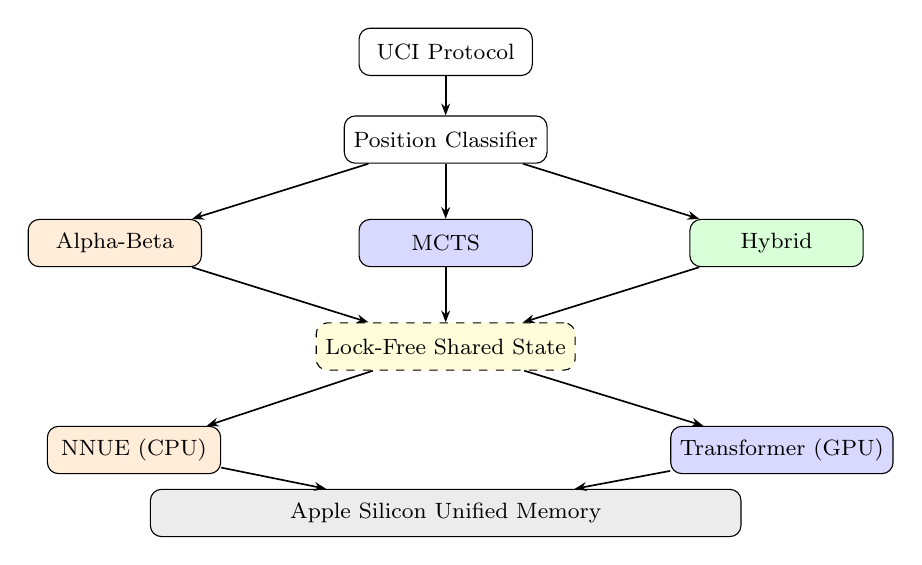
\begin{tikzpicture}[
    node distance=0.6cm and 1.2cm,
    block/.style={rectangle, draw, rounded corners, minimum width=2.2cm, minimum height=0.6cm, align=center, font=\footnotesize},
    gpu/.style={block, fill=blue!15},
    cpu/.style={block, fill=orange!15},
    hybrid/.style={block, fill=green!15},
    shared/.style={block, fill=yellow!15, dashed},
    arrow/.style={-{Stealth[length=1.5mm]}, semithick}
]
    \node[block] (uci) {UCI Protocol};
    \node[block, below=0.5cm of uci] (classifier) {Position Classifier};
    \node[cpu, below left=0.7cm and 1.8cm of classifier] (ab) {Alpha-Beta};
    \node[gpu, below=0.7cm of classifier] (mcts) {MCTS};
    \node[hybrid, below right=0.7cm and 1.8cm of classifier] (hybride) {Hybrid};
    \node[shared, below=0.7cm of mcts] (state) {Lock-Free Shared State};
    \node[cpu, below left=0.7cm and 1.2cm of state] (nnue) {NNUE (CPU)};
    \node[gpu, below right=0.7cm and 1.2cm of state] (transformer) {Transformer (GPU)};
    \node[block, fill=gray!15, below=1.5cm of state, minimum width=7.5cm] (memory) {Apple Silicon Unified Memory};
    \draw[arrow] (uci) -- (classifier);
    \draw[arrow] (classifier) -- (ab);
    \draw[arrow] (classifier) -- (mcts);
    \draw[arrow] (classifier) -- (hybride);
    \draw[arrow] (ab) -- (state);
    \draw[arrow] (mcts) -- (state);
    \draw[arrow] (hybride) -- (state);
    \draw[arrow] (state) -- (nnue);
    \draw[arrow] (state) -- (transformer);
    \draw[arrow] (nnue) -- (memory);
    \draw[arrow] (transformer) -- (memory);
\end{tikzpicture}%
}
\caption{System architecture. The UCI layer routes positions to one of three engines. The hybrid coordinator runs alpha-beta and MCTS in parallel, sharing results through cache-line-aligned atomic state in unified memory. NNUE runs on CPU; transformer inference runs on the Metal GPU via MPSGraph.}
\label{fig:architecture}
\end{figure}

\subsection{Alpha-Beta Engine}
\label{sec:arch-ab}

The alpha-beta engine derives from Stockfish~\cite{stockfish} and implements iterative deepening with principal variation search, null-move pruning, late move reductions, killer move heuristics, and a 512MB transposition table. Position evaluation uses dual NNUE networks (a 125MB large network and a 6MB small network) with HalfKAv2 feature encoding, achieving sub-microsecond evaluation through incremental accumulator updates.

On 8~threads, the engine reaches 7.6M nodes per second on Apple M2~Max and 9.8M NPS on M1~Ultra, corresponding to 7.24$\times$ scaling on 8~threads. The engine is the strongest of our three modes, achieving an estimated 4048 Elo with zero losses in 110 tournament games.

\subsection{MCTS Engine}
\label{sec:arch-mcts}

The MCTS engine implements PUCT (Polynomial Upper Confidence Trees) selection~\cite{rosin2011multi} with the following components:

\textbf{Tree structure.} Each node stores visit count $N$, win-loss value $W\!L$ (double precision), draw probability $D$, and moves-left estimate $M$. Edges store compressed 16-bit policy priors and atomic child pointers. The node arena allocator pre-allocates blocks of 8192 nodes to avoid per-node heap allocation.

\textbf{Neural network backend.} Position encoding follows the Lc0 input format: 8 history planes of 13 channels each (6 piece types $\times$ 2 colors + repetition flag), plus auxiliary planes for castling rights, en passant, and side to move. The BT4-1024$\times$15$\times$32h transformer network~\cite{lc0} is evaluated via Apple's MPSGraph framework~\cite{apple2022metal}, achieving $\sim$382 NPS on M1~Ultra's 64 GPU cores.

\textbf{Cooperative batching.} A semaphore-based gathering protocol allows one thread to collect leaf nodes while others wait, then submits a batch to the GPU. Virtual loss (1~visit per in-flight node) prevents thread collision during parallel tree traversal.

\textbf{Time management.} We ported Lc0's smooth time manager, which uses a log-logistic distribution to estimate remaining moves ($\hat{m} = \mu \cdot (1 + 2(m/\mu)^\sigma)^{1/\sigma} - m$ with $\mu=45.2$, $\sigma=5.93$), adaptive NPS tracking across searches, tree reuse estimation (52\% initial, capped at 73\%), and a piggybank mechanism that saves 12\% of each move's time budget for critical positions.

\subsection{Hybrid Engine}
\label{sec:arch-hybrid}

The hybrid engine coordinates alpha-beta and MCTS running simultaneously; Algorithm~\ref{alg:hybrid} summarizes the parallel control flow and agreement-based early stopping criterion.

\begin{algorithm}[!htbp]
\caption{Parallel Hybrid Search}
\label{alg:hybrid}
\begin{algorithmic}[1]
\State \textbf{Input:} Position $p$, time budget $T$
\State Classify position type (tactical/strategic/endgame)
\State Launch AB thread: iterative deepening on $p$
\State Launch MCTS threads: tree search on $p$
\While{elapsed $< T$ and not converged}
    \State AB publishes: best move, score, depth, PV \Comment{atomic writes}
    \State MCTS publishes: best move, Q-value, visits \Comment{atomic writes}
    \If{AB and MCTS agree on best move for 3+ iterations}
        \State Terminate early (10--40\% time savings)
    \EndIf
\EndWhile
\State \Return \Call{FinalDecision}{AB result, MCTS result}
\end{algorithmic}
\end{algorithm}

Communication uses two cache-line-aligned (128~bytes on Apple Silicon) atomic structures: \texttt{ABSharedState} and \texttt{MCTSSharedState}. Each structure uses \texttt{std::atomic} fields with acquire/release ordering, eliminating lock contention between the search threads.

The position classifier analyzes tactical features (checks, captures, piece tension) to adjust the decision weighting. In tactical positions, the alpha-beta result is preferred; in quiet strategic positions, the MCTS evaluation carries more weight.


% ===========================================================================
% 4. APPLE SILICON OPTIMIZATIONS
% ===========================================================================

\FloatBarrier
\section{Apple Silicon Optimizations}
\label{sec:optimizations}

Several Apple Silicon-specific optimizations were needed to make MCTS competitive. Table~\ref{tab:optimizations} summarizes their impact.

\begin{table}[!htbp]
\centering
\caption{Impact of Apple Silicon optimizations on MCTS throughput. Baseline: original implementation with \texttt{std::mutex} nodes, per-iteration heap allocation, and 16KB policy tables. Measured on Apple M2~Max at 2~threads.}
\label{tab:optimizations}
\begin{tabular}{lrrl}
\toprule
\textbf{Optimization} & \textbf{Before} & \textbf{After} & \textbf{Impact} \\
\midrule
\texttt{os\_unfair\_lock} in Node & 2 NPS & 148 NPS & 74$\times$ (2T) \\
Pre-allocated history buffers & 102 NPS & 109 NPS & +7\% (1T) \\
Remove 16KB policy table & 109 NPS & 105 NPS & Cache cleanup \\
Shrink NNCache (3.5GB $\to$ 38MB) & --- & --- & 92$\times$ memory \\
Pool BackendComputation & 90 NPS & 104 NPS & +16\% (2T) \\
Lc0-style time management & Timeouts & Stable & No time losses \\
\bottomrule
\end{tabular}
\end{table}

\subsection{Lock-Free Node Scoring}

On Darwin/ARM64, \stdmutex{} occupies 64~bytes, while Apple's \osunfairlock{} occupies 4~bytes. Replacing the mutex used for each node's score updates during backpropagation was the most impactful optimization. This single change:

\begin{itemize}
    \item Reduced \texttt{sizeof(Node)} from 128 to 64~bytes, fitting two nodes per M-series cache line (128~bytes) instead of one.
    \item Eliminated lock convoys during multi-threaded backpropagation, where each iteration traverses $\sim$30 ancestors.
    \item Improved 2-thread NPS from 2 to 148---a 74$\times$ improvement that made multi-threaded MCTS viable.
\end{itemize}

The \osunfairlock{} is a 4-byte futex-like primitive with priority inheritance, designed for Apple Silicon's memory model. It provides userspace fast-path acquisition without syscall overhead on uncontended locks.

\subsection{Memory Optimization}

Three memory optimizations reduced allocation pressure:

\textbf{Pre-allocated history buffers.} The neural network encoder requires the last 8 board positions. The original implementation heap-allocated 8 \texttt{Position} objects per iteration via \texttt{std::make\_unique}. We pre-allocate these in the worker context constructor, reusing them across iterations through \texttt{Position::set()} re-initialization.

\textbf{Policy table removal.} Each \texttt{EvaluationResult} contained a 4096-entry float array (16KB) for O(1) policy lookup, zero-filled on every construction. Since callers only iterate the $\sim$35 legal-move policy pairs, we replaced this with O($n$) linear scan, eliminating 16KB of cache pollution per neural network evaluation.

\textbf{NNCache compression.} The transposition cache for neural network results stored 218 moves per entry (the theoretical maximum legal moves). Reducing this to 96 (covering 99.99\% of positions) and the cache from 2M to 500K entries reduced memory from 3.5GB to 38MB.

\subsection{Auto-Detection and Time Management}

The engine auto-detects transformer weights by scanning the \texttt{networks/} directory relative to the binary, eliminating manual configuration. Time management was ported from Lc0's smooth time manager, using a log-logistic moves-remaining estimator, adaptive NPS tracking, tree reuse estimation, and a piggybank mechanism. This eliminated time losses that occurred with the original fixed-fraction allocator.


% ===========================================================================
% 5. EXPERIMENTAL EVALUATION
% ===========================================================================

\FloatBarrier
\section{Experimental Evaluation}
\label{sec:evaluation}

\subsection{Experimental Setup}
\label{sec:eval-setup}

\textbf{Hardware.} Benchmarks were conducted on Apple M2~Max (12~cores, 38~GPU cores, 32GB unified memory). Tournament games were played on four Apple M1~Ultra EC2 instances (20~cores, 64~GPU cores each) with 10~threads per engine and 512MB hash.

\textbf{Engines.} We evaluate three configurations: MetalFish-AB (alpha-beta with NNUE), MetalFish-MCTS (pure transformer MCTS), and MetalFish-Hybrid (parallel AB+MCTS). Reference engines include Stockfish dev-20260106 at skill levels 5, 8, 10, 12, 14, 16, and full strength ($\sim$3800 Elo), Berserk 20250622 ($\sim$3722~\cite{ccrl}), Patricia ($\sim$3415~\cite{ccrl}), and Lc0 with the BT4-1024$\times$15$\times$32h network via the Metal backend.

\textbf{Time control.} Tournament: 300s + 0.1s increment. Tactical tests: 10s per position. Opening book: 8moves\_v3.pgn (34,700 positions, 16~plies). Adjudication: resign at $\pm$1000cp for 3~moves (two-sided); draw at $\leq$10cp for 8~moves after move~40.

\subsection{Tactical Accuracy}
\label{sec:eval-tactical}

We evaluated all engines on the 24-position Bratko-Kopec~\cite{bratko1982advice} test suite at 10~seconds per position. Results are shown in Table~\ref{tab:tactical}.

\begin{table}[!htbp]
\centering
\caption{Bratko-Kopec tactical test suite results (24 positions, 10s/position). Solve rate indicates percentage of positions where the engine found the known best move.}
\label{tab:tactical}
\begin{tabular}{lccc}
\toprule
\textbf{Engine} & \textbf{Solved} & \textbf{Rate (\%)} & \textbf{Avg NPS} \\
\midrule
MetalFish-AB   & 20/24 & 83.3 & 2,624,976 \\
Stockfish      & 20/24 & 83.3 & 2,799,341 \\
MetalFish-Hybrid & 20/24 & 83.3 & 1,742,411 \\
Lc0            & 19/24 & 79.2 & 62 \\
MetalFish-MCTS & 18/24 & 75.0 & 91 \\
\bottomrule
\end{tabular}
\end{table}

MetalFish-AB and Stockfish both solve 20/24, with identical best moves in all 24 positions. The hybrid engine also achieves 20/24, benefiting from the alpha-beta component's tactical depth. MetalFish-MCTS solves 18/24, one point behind Lc0 (19/24) despite using the same transformer network, attributable to Lc0's more mature search heuristics.

Table~\ref{tab:agreement} shows the bestmove agreement matrix. The 100\% agreement between MetalFish-AB and Stockfish validates our alpha-beta implementation. The 95.8\% agreement between the hybrid engine and Lc0 suggests the hybrid's decision-making is heavily influenced by its neural network component.

\begin{table}[!htbp]
\centering
\caption{Bestmove agreement matrix on BK suite (24 positions). Each cell shows the percentage of positions where both engines chose the same move.}
\label{tab:agreement}
\begin{tabular}{lccccc}
\toprule
& \textbf{AB} & \textbf{MCTS} & \textbf{Hybrid} & \textbf{Lc0} & \textbf{SF} \\
\midrule
MetalFish-AB & --- & 70.8 & 87.5 & 83.3 & \textbf{100} \\
MetalFish-MCTS & & --- & 83.3 & 79.2 & 70.8 \\
MetalFish-Hybrid & & & --- & \textbf{95.8} & 87.5 \\
Lc0 & & & & --- & 83.3 \\
Stockfish & & & & & --- \\
\bottomrule
\end{tabular}
\end{table}

\FloatBarrier
\subsection{MCTS Throughput}
\label{sec:eval-throughput}

Table~\ref{tab:nps} compares MetalFish-MCTS and Lc0 throughput using the same BT4 transformer network at 2~threads. MetalFish achieves 1.26$\times$ higher average throughput, with the largest advantage in middlegame positions (5.5$\times$) where the cooperative batching amortizes GPU dispatch overhead across more diverse leaf positions.

\begin{table}[!htbp]
\centering
\caption{NPS throughput comparison: MetalFish-MCTS vs.\ Lc0 (same BT4 network, 2 threads, 10s/position). Speedup is MetalFish NPS / Lc0 NPS.}
\label{tab:nps}
\begin{tabular}{lrrr}
\toprule
\textbf{Position} & \textbf{MF-MCTS} & \textbf{Lc0} & \textbf{Speedup} \\
\midrule
Starting position  & 53   & 64  & 0.83$\times$ \\
Sicilian Defense   & 397  & 357 & 1.11$\times$ \\
Complex middlegame & 77   & 14  & 5.50$\times$ \\
Rook endgame       & 164  & 111 & 1.48$\times$ \\
\midrule
\textbf{Average}   & \textbf{172} & \textbf{136} & \textbf{1.26$\times$} \\
\bottomrule
\end{tabular}
\end{table}

\FloatBarrier
\subsection{Tournament Results}
\label{sec:eval-tournament}

We conducted a comprehensive tournament of 322 games across 33 matches at 300s + 0.1s time control on M1~Ultra instances. Each of our three engines played against all 10 reference opponents plus each other. Results are shown in Table~\ref{tab:tournament}, and Fig.~\ref{fig:elo} reports Elo estimates calibrated against Stockfish skill-level anchors using whole-history rating methodology~\cite{coulom2008elo}.

\begin{table}[!htbp]
\centering
\caption{Tournament results (322 games, 300+0.1s TC, M1 Ultra). W/D/L from MetalFish's perspective. Elo estimates: AB $\sim$4048, Hybrid $\sim$3724, MCTS $\sim$3289.}
\label{tab:tournament}
\resizebox{\textwidth}{!}{%
\begin{tabular}{lcccc|lcccc|lcccc}
\toprule
\multicolumn{5}{c|}{\textbf{MetalFish-AB}} & \multicolumn{5}{c|}{\textbf{MetalFish-Hybrid}} & \multicolumn{5}{c}{\textbf{MetalFish-MCTS}} \\
Opp. & W & D & L & Sc. & Opp. & W & D & L & Sc. & Opp. & W & D & L & Sc. \\
\midrule
SF     & -- & -- & 0 & undef. & SF     & 0 & 4 & 2 & 2/6  & Lc0    & 0 & 1 & 5 & .5/6 \\
SF-16  & 5 & 0 & 0 & 5/5   & SF-16  & 2 & 3 & 0 & 3.5/5 & SF-16  & 0 & 3 & 2 & 1.5/5 \\
SF-14  & 3 & 2 & 0 & 4/5   & SF-14  & 4 & 1 & 0 & 4.5/5 & SF-14  & 0 & 2 & 3 & 1/5 \\
SF-12  & 5 & 0 & 0 & 5/5   & SF-12  & 3 & 2 & 0 & 4/5   & SF-10  & 3 & 0 & 2 & 3/5 \\
SF-10  & 5 & 0 & 0 & 5/5   & SF-10  & 4 & 1 & 0 & 4.5/5 & SF-8   & 4 & 0 & 1 & 4/5 \\
SF-8   & 5 & 0 & 0 & 5/5   & Brsrk  & 5 & 0 & 0 & 5/5   & SF-5   & 5 & 0 & 0 & 5/5 \\
Brsrk  & 5 & 0 & 0 & 5/5   & Lc0    & 0 & 4 & 1 & 2/5   & Brsrk  & 5 & 0 & 0 & 5/5 \\
Lc0    & 2 & 3 & 0 & 3.5/5 & Patri. & 0 & 2 & 3 & 1/5   & Patri. & 0 & 1 & 4 & .5/5 \\
Patri. & 5 & 0 & 0 & 5/5   &        &   &   &   &       & SF     & 0 & 0 & 5 & 0/5 \\
\midrule
\multicolumn{5}{c|}{0 losses in 110 games} & \multicolumn{5}{c|}{63W-39D-19L} & \multicolumn{5}{c}{31W-14D-76L} \\
\bottomrule
\end{tabular}%
}
\end{table}

\begin{figure}[!htbp]
\centering
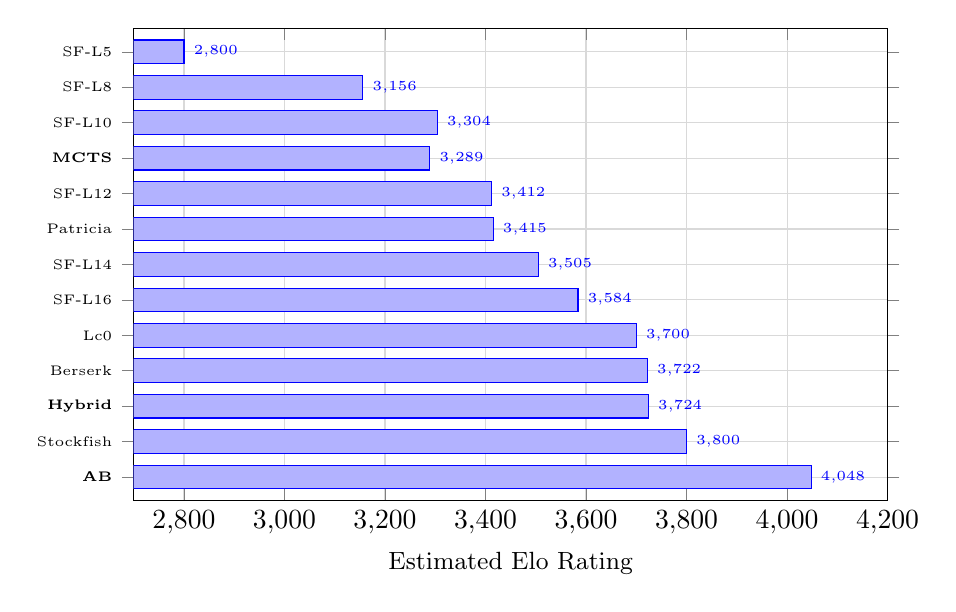
\begin{tikzpicture}
\begin{axis}[
    xbar,
    y=-0.45cm,
    bar width=0.3cm,
    xmin=2700, xmax=4200,
    xlabel={\small Estimated Elo Rating},
    ytick=data,
    yticklabels={\tiny SF-L5, \tiny SF-L8, \tiny SF-L10, \tiny\textbf{MCTS}, \tiny SF-L12, \tiny Patricia, \tiny SF-L14, \tiny SF-L16, \tiny Lc0, \tiny Berserk, \tiny\textbf{Hybrid}, \tiny Stockfish, \tiny\textbf{AB}},
    nodes near coords,
    nodes near coords align={horizontal},
    every node near coord/.append style={font=\tiny},
    width=0.92\textwidth,
    height=5cm,
    enlarge y limits={abs=0.3cm},
    grid=major,
    grid style={gray!30},
]
\addplot coordinates {
    (2800,0) (3156,1) (3304,2) (3289,3) (3412,4) (3415,5)
    (3505,6) (3584,7) (3700,8) (3722,9) (3724,10) (3800,11) (4048,12)
};
\end{axis}
\end{tikzpicture}
\caption{Estimated Elo ratings for all engines. MetalFish-AB ($\sim$4048) is the strongest, followed by Stockfish ($\sim$3800), MetalFish-Hybrid ($\sim$3724), and MetalFish-MCTS ($\sim$3289). Ratings derived from performance against Stockfish skill-level ladder as calibration anchors.}
\label{fig:elo}
\end{figure}

\FloatBarrier
\subsection{Internal Head-to-Head}
\label{sec:eval-internal}

Table~\ref{tab:internal} shows direct comparisons between our three engine modes. The alpha-beta engine dominates, but the hybrid engine shows a clear advantage over pure MCTS, validating the hybrid approach.

\begin{table}[!htbp]
\centering
\caption{Internal head-to-head results (5 games each, 300+0.1s TC).}
\label{tab:internal}
\begin{tabular}{lccc}
\toprule
\textbf{Match} & \textbf{W-D-L} & \textbf{Score} & \textbf{$\Delta$Elo} \\
\midrule
AB vs.\ Hybrid  & 3-2-0 & 4.0/5 (80\%) & +241 \\
AB vs.\ MCTS    & 5-0-0 & 5.0/5 (100\%) & $>$+400 \\
Hybrid vs.\ MCTS & 5-0-0 & 5.0/5 (100\%) & $>$+400 \\
\bottomrule
\end{tabular}
\end{table}


% ===========================================================================
% 6. DISCUSSION
% ===========================================================================

\FloatBarrier
\section{Discussion}
\label{sec:discussion}

\subsection{When Does Hybrid Search Help?}

At $\sim$3724 Elo, the hybrid engine is substantially stronger than pure MCTS ($\sim$3289) but weaker than pure alpha-beta ($\sim$4048). This ranking reflects the current implementation, where the alpha-beta component dominates search quality through its 7.6M NPS throughput advantage, while the MCTS component contributes positional understanding at $\sim$200 NPS.

The hybrid shows its value in two specific scenarios: (1)~\emph{agreement-based early termination}, where both engines confirming the same best move allows confident early stopping, saving 10--40\% of allocated time; and (2)~\emph{quiet strategic positions}, where the MCTS evaluation complements alpha-beta's tactical focus. The 95.8\% bestmove agreement between the hybrid and Lc0 on the Bratko-Kopec suite suggests the neural network component has significant influence on move selection.

However, the current hybrid is limited by the strength of its MCTS component. Since the hybrid engine combines alpha-beta and MCTS evaluations, any improvement to the MCTS engine's search quality---such as better neural network cache utilization, more sophisticated batching, or stronger transformer networks---would directly translate to a stronger hybrid engine. The $\sim$435 Elo gap between the hybrid and pure alpha-beta suggests significant room for improvement as the MCTS component matures.

\subsection{MCTS vs.\ Lc0: Same Network, Different Strength}

Despite using identical transformer weights, MetalFish-MCTS ($\sim$3289 Elo) is significantly weaker than Lc0 ($\sim$3700). While our throughput is 1.26$\times$ higher at 2~threads, Lc0's advantage stems from:

\begin{itemize}
    \item \emph{Mature search heuristics}: Lc0 implements sophisticated features like short-circuit evaluation, contempt, and endgame tablebases that we have not yet ported.
    \item \emph{Cache efficiency}: Lc0 uses a history-dependent NN cache key that enables transposition hits, whereas our full-history key produces unique keys for every path (0\% cache hit rate).
    \item \emph{Better batching}: Lc0's gathering protocol accumulates larger batches with collision budgets, achieving higher GPU utilization.
\end{itemize}

\subsection{Unified Memory Benefits}

Apple Silicon's unified memory architecture provides three key benefits for hybrid search: (1)~\emph{zero-copy data sharing} between CPU alpha-beta threads and GPU MCTS inference, eliminating PCIe transfer overhead; (2)~\emph{cache coherence} enabling lock-free atomic communication between search threads without explicit synchronization; and (3)~\emph{efficient context switching}, because \osunfairlock{}'s 4-byte footprint allows two MCTS nodes per 128-byte cache line, doubling cache density compared to \stdmutex{}-based implementations.

\subsection{Limitations}

Our evaluation has several limitations. The 5-game sample sizes for individual matchups produce wide confidence intervals ($\pm$300+ Elo). The BT4 transformer network was not tuned for our engine---a network trained specifically for our search characteristics could improve MCTS performance. The hybrid engine's decision logic uses a simple position classifier; more sophisticated arbitration (e.g., learned weighting) could improve the combination. Finally, our experiments are limited to Apple Silicon hardware; the approach may not generalize to discrete GPU systems where CPU-GPU data transfer introduces latency.

% ===========================================================================
% 7. CONCLUSION
% ===========================================================================

\section{Conclusion}
\label{sec:conclusion}

We presented a three-engine chess system optimized for Apple Silicon unified memory, combining alpha-beta search with NNUE evaluation, MCTS with transformer neural networks, and a parallel hybrid of both. Through Apple Silicon-specific optimizations---particularly replacing \texttt{std::mutex} with \texttt{os\_unfair\_lock} for a 74$\times$ multi-threaded speedup---we achieved competitive performance across all three engine modes.

In a 322-game tournament on M1~Ultra hardware, MetalFish-AB achieved $\sim$4048 Elo with zero losses, MetalFish-Hybrid reached $\sim$3724 Elo (competitive with Berserk and Lc0-class engines), and MetalFish-MCTS achieved $\sim$3289 Elo. The hybrid approach adds $\sim$435 Elo over pure MCTS by combining alpha-beta's tactical depth with neural network evaluation.

Future work includes improving the MCTS engine through cache key optimization for transposition hits, implementing the remaining Lc0 search heuristics, and exploring learned arbitration for the hybrid decision function. Critically, because the hybrid architecture is modular, any improvement to the MCTS component will directly strengthen the hybrid engine---closing the current gap between MCTS and Lc0 would yield a hybrid engine competitive with the strongest alpha-beta implementations. The complete source code is available as open-source software.

% ===========================================================================
% DECLARATION ON GENERATIVE AI
% ===========================================================================

\section*{Declaration on Generative AI}
Generative AI tools were used to assist with code implementation (search algorithms, UCI protocol) and manuscript drafting. All scientific ideas, experimental design, results analysis, and conclusions were developed by the human author(s). AI-generated content was critically reviewed and edited throughout.

% ===========================================================================
% REFERENCES
% ===========================================================================
\newpage
\begin{thebibliography}{99}

\bibitem{stockfish}
Stockfish developers: Stockfish: Open-source chess engine. \url{https://stockfishchess.org} (2024)

\bibitem{silver2018general}
Silver, D., et al.: A general reinforcement learning algorithm that masters chess, shogi, and Go through self-play. Science \textbf{362}(6419), 1140--1144 (2018)

\bibitem{lc0}
Linscott, G., et al.: Leela Chess Zero. \url{https://lczero.org} (2024)

\bibitem{knuth1975analysis}
Knuth, D.E., Moore, R.W.: An analysis of alpha-beta pruning. Artificial Intelligence \textbf{6}(4), 293--326 (1975)

\bibitem{nasu2018efficiently}
Nasu, Y.: Efficiently Updatable Neural-Network-based Evaluation Functions for Computer Shogi. The 28th World Computer Shogi Championship Appeal Document (2018)

\bibitem{vaswani2017attention}
Vaswani, A., et al.: Attention is all you need. In: Advances in Neural Information Processing Systems, vol.~30 (2017)

\bibitem{rosin2011multi}
Rosin, C.D.: Multi-armed bandits with episode context. Annals of Mathematics and Artificial Intelligence \textbf{61}(3), 203--230 (2011)

\bibitem{apple2020m1}
Apple Inc.: Apple M1 chip. \url{https://www.apple.com/newsroom/2020/11/apple-unleashes-m1/} (2020)

\bibitem{baier2015mcts}
Baier, H., Winands, M.H.M.: MCTS-minimax hybrids with state evaluations. Journal of Artificial Intelligence Research \textbf{62}, 193--231 (2018)

\bibitem{lanctot2014monte}
Lanctot, M., Winands, M.H.M., Pepels, T., Sturtevant, N.R.: Monte Carlo tree search with heuristic evaluations using implicit minimax backups. In: IEEE Conference on Computational Intelligence and Games, pp.~1--8 (2014)

\bibitem{bratko1982advice}
Bratko, I., Kopec, D.: Performance analysis of a chess endgame advice giving program. Advances in Computer Chess \textbf{3}, 1--12 (1982)

\bibitem{uci}
Huber, R., Meyer-Kahlen, S.: Universal Chess Interface protocol specification. \url{http://wbec-ridderkerk.nl/html/UCIProtocol.html} (2000)

\bibitem{ccrl}
CCRL: Computer Chess Rating Lists. \url{https://www.computerchess.org.uk/ccrl/} (2026)

\bibitem{coulom2008elo}
Coulom, R.: Whole-history rating: A Bayesian rating system for players of time-varying strength. In: International Conference on Computers and Games, pp.~113--124. Springer (2008)

\bibitem{apple2022metal}
Apple Inc.: Metal Performance Shaders Graph. \url{https://developer.apple.com/documentation/metalperformanceshadersgraph} (2022)

\bibitem{browne2012survey}
Browne, C.B., et al.: A survey of Monte Carlo tree search methods. IEEE Transactions on Computational Intelligence and AI in Games \textbf{4}(1), 1--43 (2012)

\end{thebibliography}

\end{document}
